
%%%%%%%%%%%%%%%%%%%%%%%%%%%%%%%%%%%%%%%%%%%%%%%%%%%%%%%%%%%
\section{Privacy Implications of Personal Data Processing} 
\label{sec:PrivacyImplicationsPersonalDataProcessing}
%%%%%%%%%%%%%%%%%%%%%%%%%%%%%%%%%%%%%%%%%%%%%%%%%%%%%%%%%%%


Data processing is the conversion of raw data to meaningful information through a process, where operations are performed on a given set of data to extract the required information. Data is manipulated to produce results that lead to a resolution of a problem or improvement of an existing situation. 

\ac{dm} is the process of discovering interesting patterns and knowledge from large amounts of data \cite{han2011data}. We describe the \ac{dm} process according to the widely used \ac{crisp} model \cite{wirth2000crisp} (Figure \ref{fig:crisp-dm}), in which the process is separated into six major phases, as described next.

\begin{figure}[!h]
  \centering
  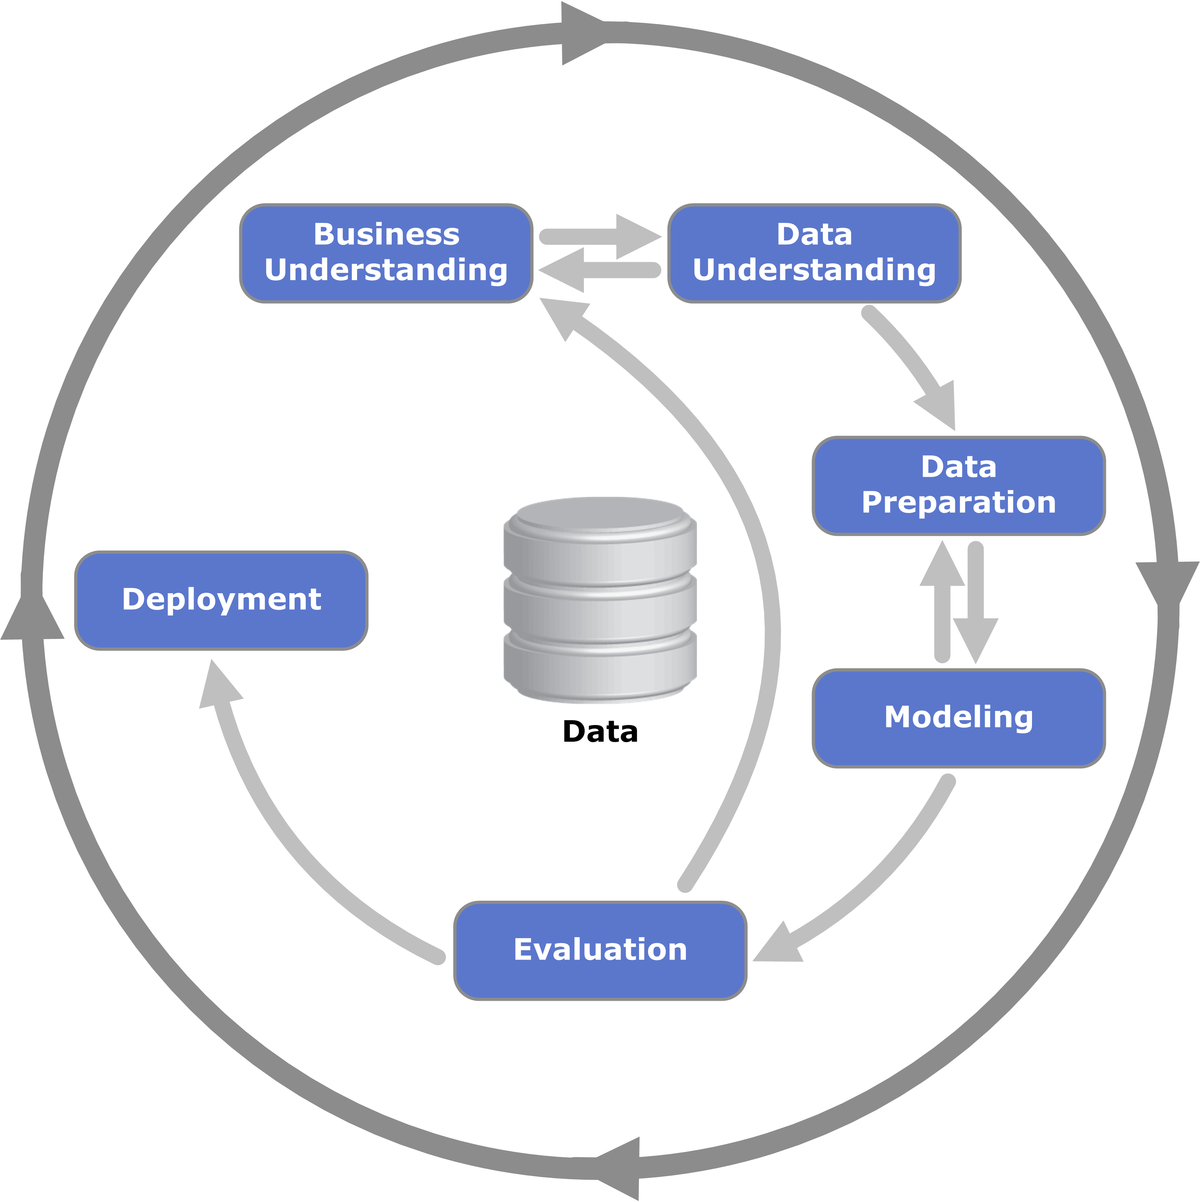
\includegraphics[width=0.60\textwidth]{images/CRISP-DM_Process_Diagram.png}
  \caption{Process diagram showing the relationship between the different phases of \acs{crisp} \cite{wirth2000crisp}.}
  \label{fig:crisp-dm}
\end{figure}

\begin{itemize}

    \item\textbf{Business Understanding:} In this initial phase, the project goals and requirements must be understood from a business perspective and then converted into a \ac{dm} problem.

    \item\textbf{Data Understanding:} During this phase, an initial data collection is done, followed by a number of activities in order to get familiar with the data, to understand how the data are organized, to identify if the data have quality problems, or even to detect interesting subsets in the data collected.

    \item\textbf{Data Preparation:} This phase covers all the data preparation tasks to construct the final dataset from the initial raw data collected. These tasks include attribute selection, data cleaning, and transformation of data to fit the modeling tools.

    \item\textbf{Modeling:} In this phase, various modeling techniques are selected and applied, and the underlying parameters are calibrated to optimal values. Usually, there are several techniques that can be applied to the same \ac{dm} problem type, and some of these techniques require specific data formats.

    \item\textbf{Evaluation:} At this point in the \ac{dm} process, one or more of the models that have been developed are excepted to be of high quality, from a data analysis perspective. These models must be evaluated thoroughly so that they properly achieve the business goals.

    \item\textbf{Deployment:} In this last phase, the knowledge gained by the \ac{dm} process needs to be organized and presented in a way that the customer can use it. This, of course, depends on the requirements presented at the beginning of the process. An example of a common deployment that results from \ac{dm} is a simple report on the knowledge obtained. 

\end{itemize}


In the \ac{dm} process, we must be aware that, sometimes, private information about individuals can be used and it may lead to breaches of privacy. We define this private information as \ac{pii} \cite{schwartz2011pii}, i.e. as information that can be used alone or in conjunction with other information to identify, contact, or locate a single person, or to identify an individual in a context.



%%%%%%%%%%%%%%%%%%%%%%%%%%%%%%%%%%%%%%%%%%%%%%
\subsection{Attack Models}
\label{ssec:AttackModels}
%%%%%%%%%%%%%%%%%%%%%%%%%%%%%%%%%%%%%%%%%%%%%%

When considering the security of a system, one must have into account the concepts of threat model, attack model, and type of adversary, to understand how to better implement an efficient and trustworthy security layer. The \textit{honest-but-curious adversary} follows the protocol, but he will try to extract information from his viewpoint to gain some form of advantage or access to confidential information.
The \textit{malicious adversary} is one that can deviate from the protocol specification as he desires, and will try to disrupt and/or collect as much information as he can.

Cryptographic attacks are possible whenever a target system relies on cryptography for protection. An attack model is, in terms of cryptanalysis, a classification of cryptographic attacks specifying the type of access the attacker has to a system when attempting to break an encrypted message. We can summarize cryptographic attacks in the following four categories:

 \begin{itemize}

    \item \textbf{Ciphertext-only attack:} In this type of attack, the adversary has access only to the ciphertext and has no access to the plaintext. This is the most common type of attack, and it is a requirement for modern ciphers to be resistant to it. An example of a ciphertext-only attack is the brute force attack, where the attacker makes a trial-and-error approach to decrypt the ciphertext.

    \item \textbf{Known-plaintext attack:} In this type of attack, the adversary has access to a number of pairs of plaintext and the corresponding ciphertext.

    \item \textbf{Chosen-plaintext attack:} In this type of attack, the adversary is able to encrypt arbitrary plaintext and have access to the resulting ciphertext, allowing him to make a statistical analysis on the plaintext state space.

    \item \textbf{Chosen-ciphertext attack:} In this type of attack, the adversary is able to choose arbitrary ciphertext and obtain the corresponding plaintext.
\end{itemize}

When designing privacy solutions using cryptography, protections must be put in place against these kinds of attacks.


